% Тут используется класс, установленный на сервере Papeeria. На случай, если
% текст понадобится редактировать где-то в другом месте, рядом лежит файл matmex-diploma-custom.cls
% который в момент своего создания был идентичен классу, установленному на сервере.
% Для того, чтобы им воспользоваться, замените matmex-diploma на matmex-diploma-custom
% Если вы работаете исключительно в Papeeria то мы настоятельно рекомендуем пользоваться
% классом matmex-diploma, поскольку он будет автоматически обновляться по мере внесения корректив
%

% По умолчанию используется шрифт 14 размера. Если нужен 12-й шрифт, уберите опцию [14pt]
\documentclass[14pt]{matmex-diploma}
%\documentclass[14pt]{matmex-diploma-custom}
\usepackage{listings}

\begin{document}
% Год, город, название университета и факультета предопределены,
% но можно и поменять.
% Если англоязычная титульная страница не нужна, то ее можно просто удалить.
\filltitle{ru}{
    chair              = {Математическое обеспечение и администрирование информационных систем},
    title              = {Создание платформы для визуализации алгоритмов YaccConstructor с помощью технологии WebSharper},
    % Здесь указывается тип работы. Возможные значения:
    %   coursework - Курсовая работа
    %   diploma - Диплом специалиста
    %   master - Диплом магистра
    %   bachelor - Диплом бакалавра
    type               = {coursework},
    position           = {студента},
    group              = 243,
    author             = {Шаламов Роман Александрович},
    supervisorPosition = {к.\,ф.-м.\,н., ст. преп.},
    supervisor         = {Григорьев С.\,В.},
%   university         = {Санкт-Петербургский Государственный Университет},
%   faculty            = {Математико-механический факультет},
%   city               = {Санкт-Петербург},
%   year               = {2013}
}
\maketitle
\tableofcontents
% У введения нет номера главы
\section*{Введение}
Возможность наглядно увидеть результат работы какого-либо алгоритма может быть очень полезной для понимания его конструкции и проведения различных тестов. В частности, очень удобно работать с алгоритмами на графах, если данные графы отрисовываются программой. 

Существует множество различных алгоритмов, которые можно визуализировать. В частности, алгоритмы проекта YaccConstructor — платформы для исследования и разработки генераторов лексических и синтаксических анализаторов и других алгоритмов для работы с грамматиками. Так как большинство алгоритмов платформы работают с грамматиками, то очень полезной может быть унифицированная технология, позволяющая выполнять отображение данных алгоритмов в графическом виде на экране пользователя. 

На данный момент в YaccConstructor уже существуют веб-приложения, выполняющие визуализацию некоторых отдельно взятых алгоритмов. Поскольку создавать для каждого алгоритма новый проект, который бы реализовывал его визуализацию -- неэффективно и трудоемко, то было принято решение о создании такого приложения, в которое можно было бы единообразно добавлять алгоритмы платформы, используя готовую библиотеку компонент и модульную архитектуру, упрощающие разработчику процесс визуализации алгоритма. 

За прототип данного приложения было решено взять кодовую базу из уже реализованных проектов (YC.BioGraph и YC.GraphParsingDemo), унифицировать её и интегрировать данные проекты как примеры работы платформы.


\section{Постановка задач}
Целью данной работы является создание единой платформы в виде веб-сайта, которая бы позволила легко реализовывать визуализацию алгоритмов YaccConstructor~\cite{yacconstructor}, а также добавление на данный сайт следующих алгоритмов: 

\begin{itemize}
\item алгоритм синтаксического анализа графов; 
\item алгоритм поиска подпоследовательностей РНК в метагеномных сборках. 
\end{itemize}

Данные алгоритмы уже представлены в виде отдельных \linebreak веб-приложений, поэтому они будут интегрированы на веб-сайт с доработкой. 


Для достижения данной цели были поставлены следующие задачи: 
\begin{itemize}
\item создание нового репозитория в YaccConstructor с названием 
    \linebreak  YC.Web с помощью технологии ProjectScaffold~\cite{prscaffold};
\item изучение особенностей фреймворка WebSharper~\cite{websharper};
\item интеграция веб-приложений (синтаксический анализ графов и поиск подпоследовательностей РНК) в YC.Web: 
    \begin{itemize}
    \item объединение кодовой базы всех алгоритмов в один проект;
    \item создание масштабируемой модульной архитектуры, позволяющей легко добавлять визуализацию новых алгоритмов;
    \item создание библиотеки общих компонент:
        \begin{itemize}
        \item компоненты ввода грамматик/графов;
        \item компонента выбора грамматик/графов из файла;
        \item компонента отрисовки графов;
        \item компоненты вывода;
        \end{itemize}
    \end{itemize}
\item добавление на сайт описания проекта YC.Web и описания работы с ним;
\item удаление репозиториев старых веб-приложений.
\end{itemize}

\section {Обзор}
YaccConstructor — это платформа для исследования и разработки генераторов лексических и синтаксических анализаторов и других алгоритмов для работы с грамматиками. Также в рамках проекта создаются и другие инструменты для работы с грамматиками, которые можно найти в репозитории на GitHub. По большей части проект реализован на языке программирования F\#.

Так как платформа YaccConstructor реализована на языке F\#, то  лучшим выбором для создания веб-приложения было использование фреймворка WebSharper.

WebSharper — это фреймворк и набор инструментов для разработки веб-приложений полностью на языках программирования C\# и F\# (или на обоих сразу). Он предоставляет как обширные серверные возможности, так и компилятор на JavaScript. Более того, с помощью него можно писать разметку веб-сайтов, используя только F\#. 

Все вышесказанное означает, что, используя WebSharper, можно создавать весь комплекс программных компонентов, используя один язык программирования, что существенно упрощает процесс разработки.

Как говорилось ранее, некоторые приложения были реализованы по отдельности различными группами разработчиков. 

 YC.BioGraph - веб-приложение для поиска подпутей в метагеномных последовательностях, которое также визуализирует полученные последовательности на исходном графе.

YC.GraphParsingDemo - веб-приложение, визуализирующее графы и соответствующие им SPPF по введенным грамматикам. Также в нем реализовано выделение минимального пути между двумя вершинами.

\section {Основная часть}
\subsection{Создание репозитория YC.Web}

Для унификации кодовой базы алгоритмов и создания модульной архитектуры  было необходимо создание общего проекта со всеми необходимыми библиотеками. 
	
Для создания репозитория использовался ProjectScaffold. 

ProjectScaffold - инструмент, предоставляющий возможности для начала работы с новом .Net/Mono проектом. Данное решения предоставляет все необходимое для успешной организации файловой системы проекта, возможности для сборки проекта на серверах, автоматическую генерацию технической документации.

В ходе работы был создан репозиторий YC.Web в организации \linebreak YaccConstrucor, подключены автоматические сборки на серверах \linebreak Appveyor(для .Net) и Travis CI(для Mono). Также была включена автоматически генерируемая документация к проекту, хостинг которой осуществляется на с помощью серверов GitHub.

\subsection{Внешний вид веб-приложения YC.Web}

YC.Web представляет собой многостраничный сайт, страницы которого можно раделить на 2 типа: основная страница (рис.~\ref{1}) и отдельные страницы для каждого из реализованных алгоритмов. (рис.~\ref{2})

\begin{figure}[h]
\label{1}
\centering
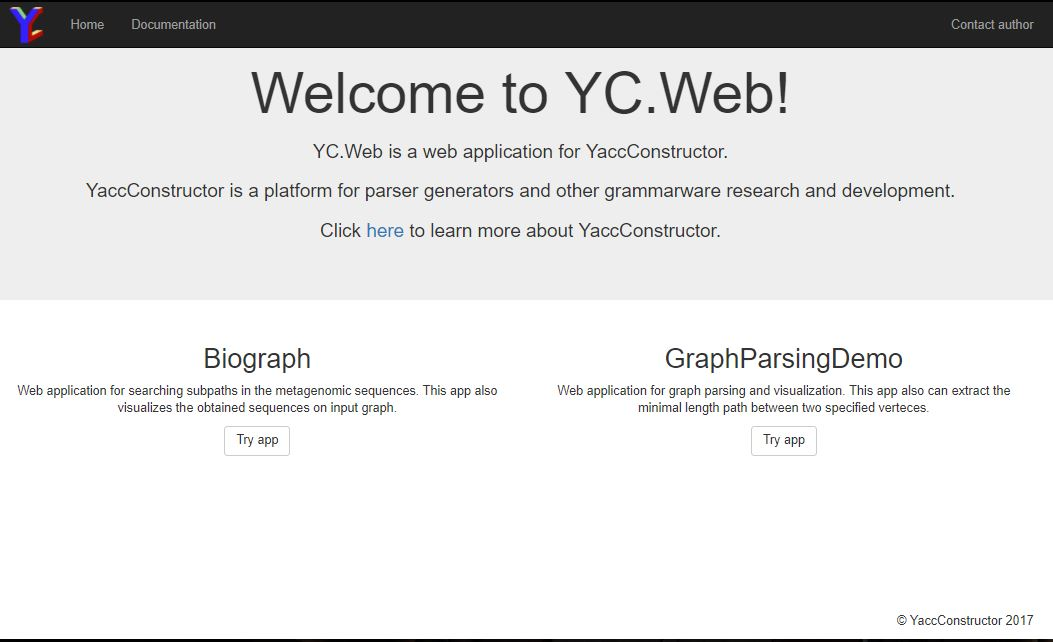
\includegraphics[width=0.9\textwidth]{pictures/main.jpg}
\caption{Главная страница YC.Web}
\end{figure}

\newpage
На основной странице присутствует краткое описание проекта \linebreak YC.Web, полезные ссылки, а также отдельные компоненты для каждого из алгоритмов, которые включают в себя название алгоритма, краткое описание алгоритма и кнопку перехода на страницу алгоритма.

\begin{figure}[h]
\label{2}
\centering
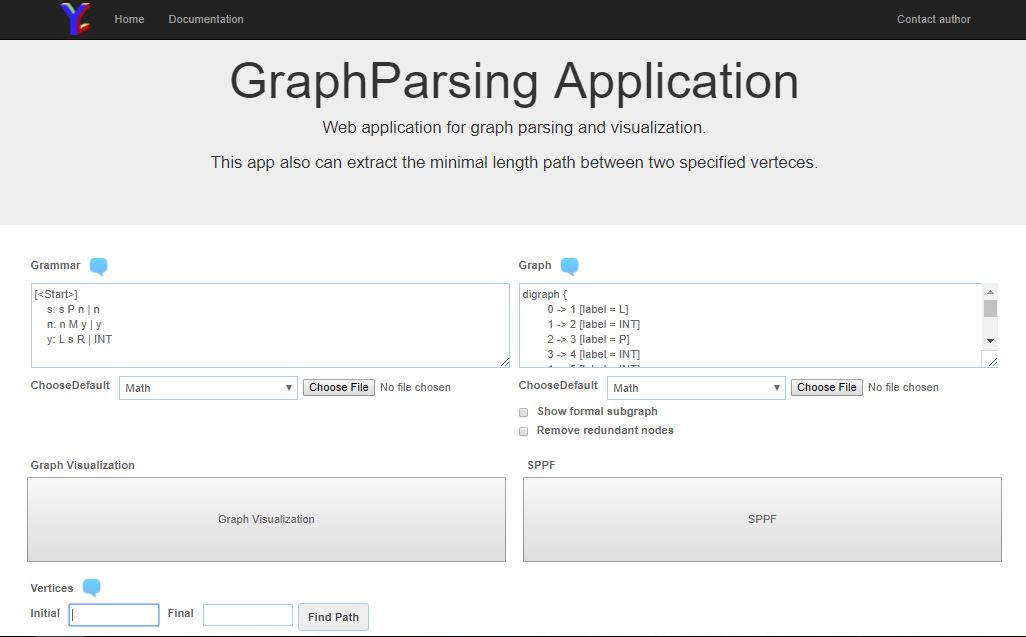
\includegraphics[width=0.9\textwidth]{pictures/alg.jpg}
\caption{Пример страницы алгоритма}
\end{figure}

\newpage

Страница каждого из алгоритмов включает в себя краткое описание алгоритма и набор из необходимых для визуализации компонент: ввод/вывод, отрисовка графа и т.п.	

Для всех страниц в проекте определено общее стилевое решение -- компонента Jumbotron библиотеки Bootstrap~\cite{bootstrap}. Данная компонента также определяет общую шапку для всех страниц веб-приложения, на которой находятся ссылки на главную страницу и документацию к проекту.

\newpage
\subsection{Структура веб-приложения YC.Web}

Как уже говорилось ранее, некоторые веб-приложения уже были реализованы как отдельные проекты. Изучив их кодовую базу были выделены следующие особенности, характерные для обоих проектов:

\begin{itemize}
    \item Все компоненты реализованы с помощью библиотеки 
    \linebreak WebSharper.Formlets, которая предоставляет набор стандартных веб-компонент (таких как ввод текста и т.д.);
    \item Компонента отрисовки графа была реализована с помощью JavaScript библиотеки Dracula.js~\cite{dracula}.
\end{itemize}


Так как в каждом из проектов вышеперечисленные технологии использовались исключительно для целей данного проекта, было принято решение реализовать общую библиотеку компонент, которая бы предоставляла возможности для независимого использования одних и тех же компонент разными проектами.

В YC.Web данная библиотека представлена в виде модуля \linebreak WebComponents, разделенного на два подмодуля: MainPageComponents и \linebreak AlgorithmsComponents. 	

Ниже представлена диаграмма данных модулей(рис.~\ref{3}).

\newpage

\begin{figure}[h]
\label{3}
\centering
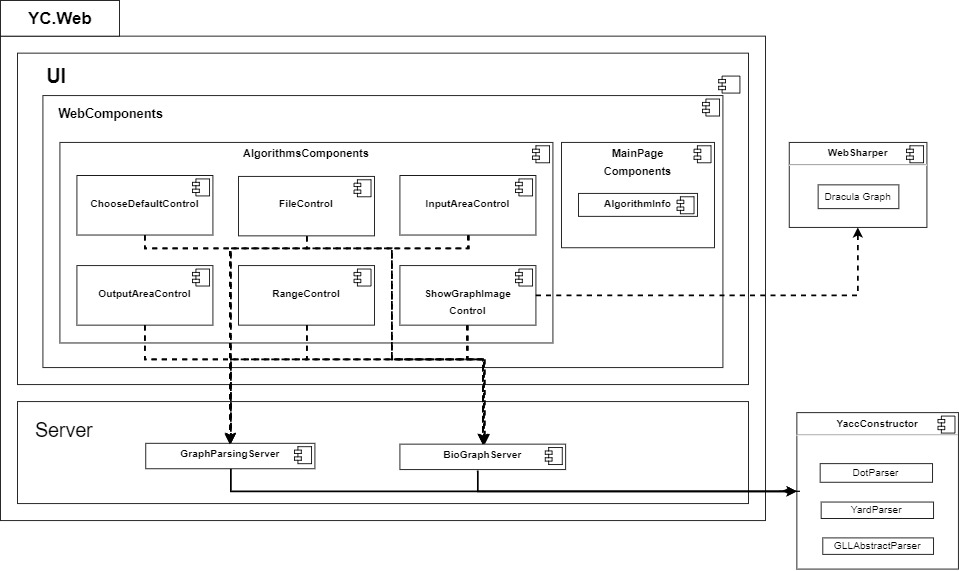
\includegraphics[width=0.9\textwidth]{pictures/modules.jpg}
\caption{Диаграмма модулей}
\end{figure}

AlgorithmComponents - библиотека компонент, используемых для  визуализации алгоритмов.

AlgorithmInfo - интерфейс для добавления нового алгоритма на стартовую страницу проекта

Модули *AlgorithmName*Functions и *AlgorithmName*Remote создаются разработчиком в отдельном файле.

*AlgorithmName*Functions - модуль, включающий в себя все необходимые для правильной работы алгоритма функции, выполняемые на сервере.

*AlgorithmName*Remote - модуль, отвечающий за клиент-серверную взаимосвязь между формами, отображаемыми на странице и функциями алгоритма.


% У заключения нет номера главы
\section*{Заключение}
В ходе данной работы были получены следующие результаты:
\begin{itemize}
    \item создан новый репозиторий с помощью технологии \linebreak ProjectScaffold под названием YC.Web;
    \item изучены особенности фреймворка WebSharper;
    \item создана модульная архитектура для добавления новых алгоритмов в YC.Web;
    \item создана библиотека общих компонент для визуализации алгоритмов;
    \item произведена интеграция следующих веб-приложений: 
        \linebreak YC.BioGraph, YC.GraphParsingDemo и удаление их старых репозиториев;
    \item на сайт с документацией было добавлено описание по работе с проектом.
\end{itemize}

В качестве дальнейшего развития возможны следующие направления: 

\begin{itemize}
    \item добавление разработчиками новых алгоритмов; 
    \item добавление новых компонент для визуализации алгоритмов;
    \item создание мобильной версии веб-приложения;
    \item интеграция репозитория с сервисом Appharbor или другим хостинг-сервисом.
\end{itemize}


\setmonofont[Mapping=tex-text]{CMU Typewriter Text}
\bibliographystyle{ugost2008ls}
\bibliography{diploma.bib}
\end{document}